
\documentclass[titlepage]{article}
\usepackage[norsk]{babel}
\usepackage[utf8]{inputenc}
\usepackage{parskip}
\usepackage{graphicx}
\usepackage{listings}

%hva som skal stå på tittelsida
\author{Gruppe 38}
\title{DB2}
\date{\today}

\begin{document}

%lager forsida
\maketitle

%man skal ha romertall på de innholdsfortegnelse
%før dette punktet skal man IKKE ha sidetall
\pagenumbering{roman}
\tableofcontents

%newpage gjør at du starter på neste side etterpå
\newpage

%herfra skal vi ha vanlige tall (arabiske (1,2,3,4,5...))
\pagenumbering{arabic}

%man pleier å starte med innledning
\section{ER-diagram}
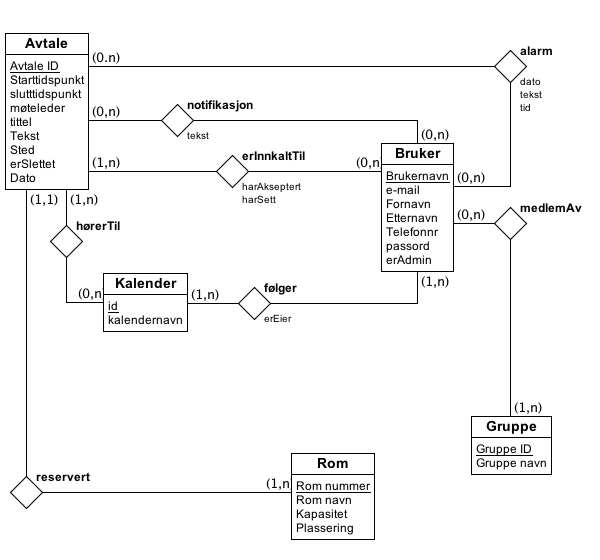
\includegraphics[width=400px]{er-diagram.png}

\newpage

\section{Kravoppfyllelse}
\paragraph{1.}\textit{ Logge på. Ansatte får tilgang til kalendersystemet ved å logge seg på kalenderklienten med brukernavn og passord:}

I ER-diagrammet har vi en brukerklasse med passordattributt. Når en bruker vil logge inn sjekker vi om brukernavnet er i databasen og at det stemmer med passordet.

\paragraph{2.}\textit{ Legge inn avtale. Ansatte skal kunne legge inn avtaler i kalenderene sine. En avtale
legges inn på avtaledato med et start- og sluttidspunkt, samt en kort beskrivelse av
avtalen (``Bil på verksted'') og eventuelt sted for avtalen (``Strandveien Auto''):}

Da oppretter man et objekt av avtale-entiteten som inneholder start- og sluttidspunkt. Man kan også velge om man skal reservere et rom eller legge til et sted. Sted viser om hva man har reservert.

\paragraph{3.}\textit{ Slette avtale. Ansatte skal kunne slette en avtale som ligger i en av kalenderene sine.}

Da sletter man bare avtalen med den gjeldene ID en. Entiteter som hører til avtalen lytter på handlingen og oppdaterer seg.

\paragraph{4.}\textit{ Endre avtale. Ansatte skal kunne endre på en avtale som ligger i en av kalenderene sine. Alle feltene kan endres.}

En bruker kan redigere en kalender der har-relasjonen mellom bruker og kalender har ‘erEier’ feltet satt til sant. 

\paragraph{5.}\textit{ Kalle inn til møte. En ansatt skal kunne kalle andre ansatte og grupper i Firma X inn til et møte. Den som kaller inn til møte kalles en møteleder. En ansatt skal kunne kalle inn til møte på samme måte som han/hun legger ny avtale inn i en kalender. I tillegg til
feltene for en vanlig avtale, inneholder også møteinnkallingen en liste over innkalte
møtedeltakere.}

Når en ansatt oppretter en avtale så blir han satt til møteleder uansett. Den ansatte kan da også invitere med andre brukere med ‘Er innkalt til’ relasjonen. Hvis han kaller inn en gruppe til møte, så vil systemet gå igjennom gruppens medlemmer og gi de individuelle innkallinger slikt som enkelt personer blir innkalt. 

I avtale får man også tilgang til tidligere inviterte medlemmer og hva statusen på invitasjonen er. 


\paragraph{6.}\textit{ Motta møteinnkalling. Når en ansatt mottar innkalling til et møte, kan han/hun svare
'Godta' eller 'Forkast'. Ved å svare 'Godta', legges møteinnkallingen inn som en avtale
i den innkalte ansattes kalender. Om den ansatte svarer 'Avslag', sendes svar tilbake til
møtelederen om at innkallingen ikke er godtatt. Møteleder kan da velge å finne et nytt
tidspunkt, avlyse møtet (se under) eller fjerne deltakeren fra innkallingslista.}

Dersom brukeren svarer godta/avslå vil dette bli lagret som en relasjon mellom brukeren og avtalen. På denne måten holder vi styr på hvilke møter brukern skal vise i kalenderen. Vi holder også styr på hvem som er møteleder slik at han kan redigere møte. Et møte er koblet opp mot en dag som igjen er det som vises i kalenderen. Når man blir kalt inne til et møte vil brukeren motta en notifikasjon.


\paragraph{7.}\textit{ Endre møteinnkalling. Møteleder kan endre tidspunkt på en møteinnkalling. Det
sendes da beskjed ut til alle møtedeltakerne, som kan svare 'Godta' eller 'Forkast'. Ved
å svare 'Godta', endres avtalen i den innkalte ansattes kalender. Ved å svare 'Forkast'
sendes beskjed ut til alle innkalte møtedeltakere. Møteleder kan da velge å finne et
nytt tidspunkt eller å avlyse møtet (se under).}

Ettersom vi holder styr på hvem som er møteleder kan han redigere informasjon om møte. Når han endrer et møte kan han sende ut ny notifikasjon til brukerne som de kan svare på. Dersom brukere skulle svare forkast blir det sendt ut en ny notifikasjon til alle brukerne.

\paragraph{8.}\textit{ Avlyse møte. Møteleder kan avlyse et møte. Det sendes da beskjed til alle
møtedeltakerne, og systemet sletter møtet i deltakernes personlige kalender.}
Vi oppretter en notifikasjon mot alle ansatte som er innkalt til møtet som forteller at møtet er avlyst. Deretter setter vi erSlettet verdien i møtet til sant. Når de innkalte brukerene får den nye notifikasjonen samt nye dataene om møtet så vil systemet se at ‘erSlettet’ er satt til sant og dermed vil ikke møtet vises lengre.

\paragraph{9.}\textit{ Melde avbud for møte. En ansatt kan melde avbud på en møteinnkalling ved å slette avtalen i sin personlige kalender. Når en ansatt melder avbud, sendes melding til alle de andre møtedeltakerne. Møteleder kan da velge om møtet skal avlyses eller om
han/hun skal endre tidspunkt på møtet.}

En ansatt kan forandre statusen sin til møte til at erGodtatt blir false, dermed blir det lagret i systemet at møtet ikke skal vises i kalenderen til brukeren. Dermed kan møteleder få beskjed slik at han kan slette møte som bare føres til at møte hides i databasen, eller redigere informasjonen.










\paragraph{10.}\textit{ Reservere møterom. I stedet for å skrive inn sted for en avtale eller et møte, skal brukeren kunne reservere møterom. Kalendertjeneren skal lage en liste med
tilgjengelige møterom (tilgjengelig betyr ikke reserverte) i tidsperioden for
avtalen/møtet. Brukeren kan da velge møterom fra denne listen. Om en avtale med
reservert møterom slettes, skal reservasjonen slettes på kalendertjeneren. Det samme
gjelder for møter som avlyses.}

Gjør først en spørring etter alle rom som er opptatt i den gjeldene tidsperioden og fjerner disse fra listen over alle rom skal bli vist til brukeren. Da står vi igjen med alle de ledige rommene og valgt rom vil bli lagret i avtaleentiteten. Dersom en avtal blir slettet vil relasjonen forsvinne og rommet vil ikke lenger være opptatt.

\paragraph{11.}\textit{ Visning. Kalenderklienten skal vise en ukekalender der alle avtaler og møter i den ansattes personlige kalender vises. Det skal være enkelt å bla mellom ukene.}

Når vi skal hente ut ukekalenderen gjør vi bare en spørring på alle avtaler i gjeldene kalendere til brukeren, i det gjeldene tidsrommet.

\paragraph{12.}\textit{ Spore møteinnkallinger. Kalenderklienten skal indikere i ukekalenderen om a) en
møteinnkalling venter på svar fra en eller flere deltakere, b) en eller flere
møtedeltakere har avslått møteinnkalling, eller c) om alle innkalte har godtatt
møteinnkallingen.}
\subparagraph{a)} ‘Er innkalt til’ relasjonen mellom Avtale og Bruker vil vise hvor mange som ikke har sett/ svart på innkallingen.

\subparagraph{b)} ‘Er innkalt til’ relasjonen mellom Avtale og Bruker vil vise hvor mange som har avlsått innkallingen.

\subparagraph{c)} ‘Er innkalt til’ relasjonen mellom Avtale og Bruker vil vise hvor mange som har godtatt innkallingen.

\paragraph{13.}\textit{ Vis flere kalendre. Det skal være mulig å vise andre ansattes avtaler sammen med sine
egne i kalenderklienten.}

En bruker kan kobles opp mot flere kalendere som tilhører andre brukere.


\paragraph{14.}\textit{ Alarm. Det skal være mulig for hver ansatt å konfigurere enhver avtale slik at avtalen
genererer en alarm en gitt tid før møtet.}

Alarm er en relasjon mellom avtale og bruker. En bruker kan dermed ha flerer alarmer til flere møter. Relasjonen inneholder et dato felt som sier når alarmen skal utløses.

\end{document}
